\documentclass[11pt,a4paper]{report}
\usepackage{amsmath}
\usepackage{amssymb}

\usepackage{graphicx}

\usepackage{listings}
\usepackage{color} %red, green, blue, yellow, cyan, magenta, black, white
\definecolor{mygreen}{RGB}{28,172,0} % color values Red, Green, Blue
\definecolor{mylilas}{RGB}{170,55,241}


\usepackage{graphicx}


\begin{document}
\begin{center}

\LARGE Adjoint Equation


\end{center}
\textbf{General problem}
\\
Looking at an optimal control problem $$\underset{y,u}{\text{min}} \ J(y,u) \ \text{subject to} \ E(y,u)=0$$ Where $u \in U$ is the control and $y \in Y$ is the state that depends on $u$. Usually $u$ and $y$ are functions, and $U$ and $Y$ are either Hilbert or Banach spaces. I will not go into detail about these spaces, but they are mostly chosen to fit the differential equation $E$, which is an operator on $U\times Y$.
\\
\\
Differentiating $J$ is required for solving the problem. To do this we reduce $J$ to $\hat{J}(u) = J(y(u),u) $ and compute its gradient in direction $s \in U$. Will use the notation: $\langle\hat{J}'(u),s\rangle$ for the gradient.
\begin{align*}    
\langle\hat{J}'(u),s\rangle &= \langle\frac{\partial J(y(u),u)}{\partial u},s\rangle \\ &= \langle \frac{\partial y(u)}{\partial u}^*J_y(y(u),u),s\rangle + \langle J_u(y(u),u),s\rangle \\ &= \langle y'(u)^*J_y(u),s\rangle +\langle J_u(u),s\rangle
\end{align*}
Here $\langle\cdot,\cdot\rangle$ is the $U$ inner product. The difficult term in the expression above is $y'(u)^*$, so lets first differentiate $E(y(u),u)=0$ with respect to $u$, and try to find an expression for $y'(u)^*$: 
\begin{align*}
\frac{\partial}{\partial u}E(y(u),u)=0 &\Rightarrow E_y(y(u),u)y'(u)=-E_u(y(u),u) \\ &\Rightarrow y'(u)=-E_y(y(u),u)^{-1}E_u(y(u),u) \\ &\Rightarrow y'(u)^* = -E_u(y(u),u)^*E_y(y(u),u)^{-*}
\end{align*} 
By inserting our new expression for $y'(u)^*$ into $y'(u)^*J_y(u)$, we get:
\begin{align*}
y'(u)^*J_y(u)&=-E_u(y(u),u)^*E_y(y(u),u)^{-*}J_y(u) \\
&=-E_u(y(u),u)^*p
\end{align*}
$\lambda$ is here the solution of the adjoint equation 
\begin{gather*}
E_y(y(u),u)^{*}p=J_y(u)
\end{gather*}
If we can solve this equation for $\lambda$, the gradient of $\hat{J}$ will be given by the following formula:  
\begin{gather}
\langle\hat{J}'(u),s\rangle=\langle -E_u(y(u),u)p,s\rangle +\langle J_u(u),s\rangle
\end{gather} 
\\
\\
\textbf{Optimal control with ODE constraints}
\\
\\
Lets try to derive the adjoint equation and the gradient, when we let $E(y,u)$ be the following ODE:
\begin{align*}
\left\{
     \begin{array}{lr}
       	y'(t)=\alpha y(t) +u(t), \ t \in (0,T)\\
       	   y(0)=y_0
     \end{array}
   \right.
\end{align*}
We also choose the functional to be
\begin{align*}
J(y,u) = \frac{1}{2}\int_0^Tu(t)^2dt + \frac{1}{2}(y(T)-y^T)^2
\end{align*}
Before we calculate the different terms in the gradient, we want to fit our ODE into an expression $E$. we do this by "moving" the initial condition into the equation:
\begin{align*}
E(y,u) = y'-\alpha y - u + \delta_0(y-y_0)
\end{align*}
Here the $\delta_0$ means evaluation at $0$. Now  lets find $E_u$, $E_y$, $ \langle J_u(u),s\rangle$ and $J_y$ with respect to our $E$ and $J$.
\begin{align*}
E_u(y(u),u)&=-1 \\
E_y(y(u),u)&=\frac{\partial}{\partial t} - \alpha + \delta_0 \ \text{,where $\delta_0$ is evaluation at 0} \\
\langle J_u(u),s\rangle &= \int_0^T u(t)s(t) dt 
\end{align*}
Lets be more thorough with $J_y$, which is the right hand side in the adjoint equation.
\begin{align*}
J_y(y(u),u) &= \frac{\partial}{\partial y}(\frac{1}{2}\int_0^Tu^2dt + \frac{1}{2}(y(T)-y^T)^2) \\ &= \frac{\partial}{\partial y} \frac{1}{2}(y(T)-y^T)^2 \\
&= \frac{\partial}{\partial y}\frac{1}{2}(\int_0^T \delta_T(y-y^T)dt)^2 \\
&= \delta_T\int_0^T \delta_T(y(t)-y^T)dt \\
&= \delta_T(y(T)-y^T)=L
\end{align*}
We have $E_y(y(u),u)=\frac{\partial}{\partial t} - \alpha + \delta_0$, but for the adjoint equation we need to find $E_y^*$.
To derive the adjoint of $E_y$, we will apply it to a function $v$ and then take the $L^2$ inner product with another function $w$. The next step is then to try to "move" the operator $E_y$ from $v$ to $w$. As becomes clear below, partial integration is the main trick to achieve this: 
\begin{align*}
\langle E_yv,w \rangle &=  \int_0^T(v'(t)-\alpha v(t)+\delta_0v(t))w(t)dt \\ &= \int_0^Tv'(t)w(t)dt -\alpha\int_0^Tv(t)w(t) dt +v(0)w(0) \\
& = -\int_0^Tv(t)w'(t)dt +v(t)w(t)|_0^T-\alpha\langle v,w\rangle +v(0)w(0) \\
&=-\int_0^Tv(t)w'(t)dt -\alpha\langle v,w\rangle +v(T)w(T) \\
&= \langle v,Pw \rangle
\end{align*} 
Where $P=-\frac{\partial}{\partial t} -\alpha + \delta_T$. This means that $E_y^* = P$, and we now have the left hand side in the adjoint equation. The right hand side is $J_y(y(u),u)=L$, which we have already found. If we write the  adjoint equation on variational form it will look like this: $\langle Pp,w\rangle = \langle L,w\rangle$. To get back to standard ODE form, we can do some manipulation: 
\begin{align*}
\langle -p'-\alpha p +\delta_T p,w \rangle &= \langle \delta_T(y(T)-y^T),w\rangle \\
\langle -p'-\alpha p ,w \rangle &= \langle \delta_T(y(T)-y^T -p),w\rangle
\end{align*}
The right hand side is point evaluation at $t=T$, while the left hand side is an expression for all $t$. This finally gives us our adjoint equation: 
\begin{align*}
   \left\{
     \begin{array}{lr}
       -p'(t) = \alpha p(t) \\
       p(T) = y(T)-y^T
     \end{array}
   \right.
\end{align*}
This is a simple and easily solvable ODE.
\\
\\
\textbf{Expression for the gradient}
\\
We now have all the ingredients for finding an expression for the gradient of $\hat{J}$. If we remember that $\langle\hat{J}'(u),s\rangle=\langle y'(u)^*J_y(u),s\rangle +\langle J_u(u),s\rangle$, and all the different expressions for all the terms we calculated, we find:
\begin{align*}
\langle\hat{J}'(u),s\rangle&=\langle y'(u)^*J_y(u),s\rangle +\langle J_u(u),s\rangle \\ &=\langle -E_u^*p,s\rangle +\langle J_u(u),s\rangle \\
&=\langle -(-1)^*p,s\rangle +\langle u,s\rangle \\
&=\langle p+u,s\rangle \\
&= \int_0^T(p(t)+u(t))s(t)dt
\end{align*} 
Note that the adjoint of a constant is just the constant itself.
\\
\\
\textbf{Parallelizeing in time using the penalty method}
\\
To find the above gradient, we must solve first the state equation forward in time and then the adjoint equation backwards in time. One way of speeding things up is to parallelize the solvers by partitioning the time interval and then solving the equation separately on each partitioned interval. If we split the interval $[0,T]$ into $m$ parts we need to solve $m$ state equations on the following form:
\begin{align*}
   \left\{
     \begin{array}{lr}
       \frac{\partial }{\partial t} y_i(t) = \alpha y_i(t) + u(t) \ \text{for $t \in [T_{i-1},T_{i}]$}\\
	y_i(T_{i-1}) = \lambda_{i-1}
     \end{array}
   \right.
\end{align*}
here $i=1,...,m$, $\lambda_0=y_0$ and $0=T_0<T_1<\cdots<T_{m}=T$. Since the equation on each interval depends on the equation in the previous interval, we need a trick, to get everything to hang together. We do this using the penalty method, which means adding a penalty to the functional. The new functional now looks like this:
\begin{align*}
J(y,u,\lambda) = \int_0^T u^2 dt + \frac{1}{2}(y_m(T)-y^T)^2 + \frac{\mu}{2} \sum_{i=1}^{m-1} (y_{i}(T_i)-\lambda_i)^2 
\end{align*}
This means that the problem now is to minimize $J$ with respect to both $u$ and $\lambda$, which means that the reduced functional depends on both $u$ and $\lambda$. Since we change the functional and the equation, both the adjoint equation and the gradient changes. Lets try to derive the new adjoint equations and the new gradient. The gradient of the reduced functional now looks like the following:
\begin{align*}
\langle \hat{J}'(u,\lambda), (s,l)\rangle &= \langle \frac{\partial y(u,\lambda)}{\partial(u,\lambda)}^* J_y(y(u,\lambda),u,\lambda), (s,l)\rangle + \langle J_u+J_{\lambda}, (s,l)\rangle \\
&=\langle -(E_u+E_{\lambda})p , (s,l)\rangle + \langle J_u+J_{\lambda}, (s,l)\rangle
\end{align*} 
Where p is the solution of the adjoint equation $E_y^*p=J_y$, and $E$ is our ODEs:
\begin{align*}
E^i(y,u,\lambda)= \frac{\partial }{\partial t} y_i - \alpha y_i -u+ \delta_{T_{i-1}}(y_i-\lambda_{i-1})
\end{align*} 
Lets differentiate $E$:
\begin{align*}
E_y^i &= \frac{\partial }{\partial t} - \alpha + \delta_{T_{i-1}} \\
E_u^i &= -1 \\
E_{\lambda_{i-1}}^i &= -\delta_{T_{i-1}} \ \text{for $i=2,...,m$}
\end{align*}
Lets differentiate $J$:
\begin{align*}
\langle J_u,s\rangle &= \int_0^T us \ dt \\
J_{\lambda_i}&= -\mu(y_{i}(T_i)-\lambda_i) \\
J_y &= \delta_{T_{m}}(y_n(T_{m})-y_T) + \mu \sum_{i=1}^{m-1} \delta_{T_{i}}(y_{i}(T_i)-\lambda_i ) 
\end{align*}
We also need $(E_y^i)^*$
\begin{align*}
\int_{T_{i-1}}^{T_{i}} E_y^iw \ v \ dt & = \int_{T_{i-1}}^{T_{i}} (\frac{\partial }{\partial t}w -\alpha w) \ v \ dt + w(T_{i-1})v(T_{i-1}) \\
&= \int_{T_{i-1}}^{T_{i}}-(\frac{\partial }{\partial t}v+\alpha v) \ w \ dt + w(T_{i})v(T_{i}) \\
&= \int_{T_{i-1}}^{T_{i}} (-\frac{\partial }{\partial t}-\alpha + \delta_{T_{i}})v \ w \ dt
\end{align*} 
this means that $(E_y^i)^*=-\frac{\partial }{\partial t}-\alpha + \delta_{T_{i}}$. This gives us the following expressions for the adjoint equations:
\\
\\
$i=n$ case:
\begin{align*}
-\frac{\partial }{\partial t}p_m &=\alpha p_m  \\
p_m(T_{m}) &= y_m(T_{m})-y_T
\end{align*}
$i\neq m$ cases:
\begin{align*}
-\frac{\partial }{\partial t}p_i &=p_i  \\
p_i(T_{i}) &= \mu(y_{i}(T_{i})-\lambda_{i} )
\end{align*}
Lets put everything into our expression for or gradient:
\begin{align*}
\langle \hat{J}'(u,\lambda), (s,l)\rangle&=\langle -(E_u+E_{\lambda})p, (s,l)\rangle + \langle J_u+J_{\lambda}, (s,l)\rangle \\
&= \langle (p+\sum_{i=1}^{m-1} \delta_{T_i}p_{i+1}) , (s,l)\rangle+ \int_0^T us \ dt - \mu \sum_{i=1}^{m-1}(y_{i}(T_i)-\lambda_i)l_i\\
&=\int_0^T (u+p)s \ dt +\sum_{i=1}^{m-1}(p_{i+1}(T_i) -\mu(y_{i}(T_i)-\lambda_i) )l_i \\
&= \int_0^T (u+p)s \ dt +\sum_{i=1}^{m-1}(p_{i+1}(T_i) -p_{i}(T_i) )l_i
\end{align*} 
\\
\\
\textbf{Simple example}
\\
Let $T=y_T=y_0=\alpha=1$ and assume that we want to find the gradient of $\hat{J}$ at $u(t)=0$. We then have:
\begin{gather}
J(y,u) = \frac{1}{2}\int_0^1u^2dt + \frac{1}{2}(y(T)-1)^2
\end{gather} 
and
\begin{align}
\left\{
     \begin{array}{lr}
       	y' =  y +u\\
       	   y(0)=1
     \end{array}
   \right.
\end{align}
Since $u=0$, we easily find $y(t)=e^t$. This gives us the adjoint equation:
\begin{align}
   \left\{
     \begin{array}{lr}
       -p'(t) -p(t)=0  \\
       p(T) = e-1
     \end{array}
   \right.
\end{align}
This is again a simple equation which yields $p(t)=(e-1)e^{1-t}$. The gradient of $\hat{J}$ is then:
\begin{align*}
\langle\hat{J}'(u),s\rangle=\int_0^1(e-1)e^{1-t}s(t)dt
\end{align*}
\\
\\
\textbf{Discretization}
\\
Let us discretize our interval $[0,T]$ using $N+1$ points where 
\begin{align*}
x_n &= n\Delta t, \ i=0,...,N \ \text{ and} \\
\Delta t &= \frac{T}{N}
\end{align*}
We also let $y^n = y(x^n)$ and $u^n=u(x^n)$. The integrals in our functional and its gradient we evaluate using the trapezoidal rule, and we discretize our ODE $E(y,u)=0$ and the adjoint equation using the Backward Euler scheme. For $E(y,u)=0$ we get :
\begin{align*}
\frac{y^n-y^{n-1}}{\Delta t} &= \alpha y^{n} + u^{n} \\
(1-\alpha\Delta t)y^{n} &= y^{n-1} +\Delta t u^{n} \\
y^n &=\frac{y^{n-1} +\Delta t u^{n}}{1-\alpha\Delta t}
\end{align*} 
Here the initial condition $y^0=y_0$ is known. For the adjoint equation the initial condition is $\lambda^N = y^N-y^T $, and the Backward Euler scheme gives us:
\begin{align*}
-\frac{p^n-p^{n-1}}{\Delta t} -\alpha p^n &=0 \\
p^{n-1} -p^n &=\Delta t\alpha p^n \\
p^{n-1} &= (1+\Delta t\alpha)p^n
\end{align*}
\\
\\
\textbf{The discrete gradient}
\\
So we now have a way of solving our ODEs numerically. In the continuous case the gradient was $\int_0^T(p(t)+u(t))s(t)dt$, however in the discrete case, $\hat{J}$ is a function dependent on the $N+1$ values of $u$. This would suggest that the gradient of $\hat{J}$ should be a vector of size $N+1$. The thing that makes the most sense to me is to insert the unit vectors of $\mathbb{R}^{N+1}$ into our continuous gradient, and then evaluate the integral using the trapezoidal rule. Based on experiments using finite difference for calculating $\hat{J}$, this approach works for $n\neq 0$ and $n\neq N$. Without more explanation I will assert that our discrete gradient $\hat{J}'_{\Delta t}(u)$ looks like this:
\begin{align*}
\hat{J}'_{\Delta t}(u)^n&=\Delta t(u^n+p^n) \ \text{when $n=1,...,N-1$} \\
\hat{J}'_{\Delta t}(u)^0&=\Delta t \frac{1}{2}u^0 \\
\hat{J}'_{\Delta t}(u)^N&=\Delta t(\frac{1}{2}u^N+p^N)
\end{align*} 
Lets try to understand what happens for $n=0$ and $n=N$. For $n=0$ we see that there is no $p$ term. This is because $y$ does not depend on $u(0)$. The reason that this matters in the discrete case and not in the continuous case, is that the point $t=0$ has measure zero, and the continuous gradient is an integral. We also notice the $\frac{1}{2}$ term in front off $\Delta t u^0$. This comes from our numerical integration using the trapezoidal rule. To make this clear lets state the trapezoidal rule:
\begin{align*}
\int_0^1 f(t)dt \approx \Delta t[\frac{f^0+f^N}{2}+\sum_{n=1}^{N-1}f^n]
\end{align*} 
Looking at this expression we also understand the $n=N$ case. Also note that integrating over $(p + \frac{1}{2}u)e^N$ using the trapezoidal rule would give us an extra factor of $\frac{1}{2}$ that is not there when we use finite difference for $\hat{J}'(u)$. This Will all be demonstrated below. One could perhaps derive the discrete results by translating the functional and the ODE to discrete setting , where you exchange $L^2(\Omega)$ with $\mathbb{R}^{N+1}$, but I will not do this now. 
\\
\\
\textbf{Testing numerics with simple example}
\\
Want to test the numerical adjoint to the exact adjoint for the simple example I did above, i.e. $T=y_T=y_0=\alpha=1$ and $u=0$. This gave us the the following solution to our adjoint equation: $p(t)=(e-1)e^{1-t}$. Using the finite difference schemes I derived above, I calculated the maximum difference between the exact and the numerical adjoint for $N=\{50,100,500,1000 \}$ points. The results of the experiment is added in the table below: 
\begin{center}
    \begin{tabular}{| l | l | l | l | l |}
    \hline
    N & 50 & 100  & 500 & 1000 \\ \hline
    max($|p^n-p(t^n)|$) & 0.0317 &0.0156&0.0031 &0.0015 	\\ \hline
    \end{tabular}
\end{center}
Using least squares we can find the convergence rate of $|p^n-p(t^n)|$ in $\Delta t$, and as expected using simple backward Euler, we get linear convergence: 
\begin{align*}
|p^n-p(t^n)|_{\infty} \leq \Delta t C
\end{align*}
In this case $C\approx1.7$. I have also added a plot of the exact and numerical adjoints for $N=50$.
\begin{figure}
  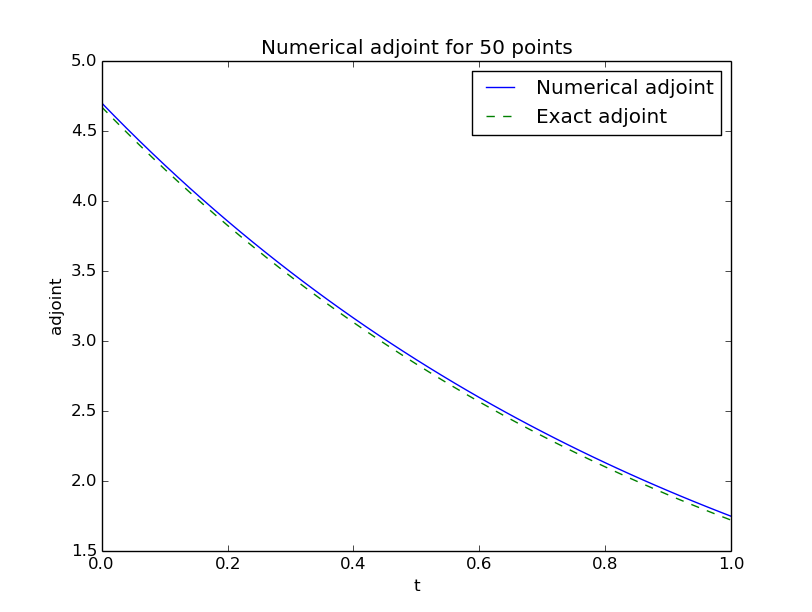
\includegraphics[width=\linewidth]{adjoint_plot.png}
  \caption{Adjoint for $u=0$ and $T=y_T=y_0=\alpha=1$}
  \label{Fig 1}
\end{figure}
\\
\\
\textbf{Testing gradient using finite difference}
\\
Now lets try to test the claims I made earlier about the discrete gradient. I will approximate the gradient using finite difference in the following way:
\begin{align*}
&\hat{J}'(u)^n \approx \frac{\hat{J}(u+\epsilon^n)-\hat{J}(u)}{\epsilon} \\
&\epsilon^n=\epsilon e^n \in \mathbb{R}^{N+1} \ \text{with $\epsilon>0$ small, and $e^n$ the unit vector}
\end{align*} 
As always I let $T=y_T=y_0=\alpha=1$, however this time I choose $u(t)=e^t+t$. I then define the relative error E between the discrete adjoint gradient $\hat{J}'_{\Delta t}(u)$ and the finite difference gradient $\hat{J}'_{\epsilon}(u)$ defined as:
\begin{align*}
E=|\frac{\hat{J}'_{\Delta t}(u)-\hat{J}'_{\epsilon}(u)}{\Delta t}|_{\infty}
\end{align*}
I use this error to test the gradients for different $N$. The result is given in a table below, and I have also added a plot. Note that I as last time calculated convergence rate using least squares, and the result was: $E\leq \Delta tC$, with $C\approx27$.
\begin{center}
    \begin{tabular}{| l | l | l | l | l |}
    \hline
    N & 50 & 100  & 500 & 1000 \\ \hline
    E & 0.5658 &0.2816 &0.0561 & 0.0281	\\ \hline
    \end{tabular}
\end{center}
\begin{figure}
  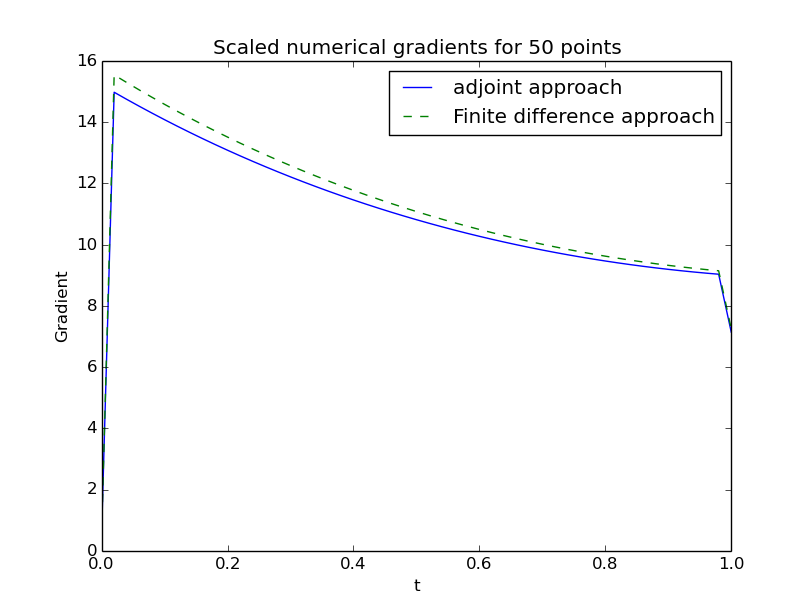
\includegraphics[width=\linewidth]{finite_diff_plot.png}
  \caption{"Relative" gradients for $u=0$ and $T=y_T=y_0=\alpha=1$}
  \label{Fig 2}
\end{figure}
\textbf{Testing manufactured solution to control problem}
\\
We now know how to create the gradient of a simple optimal ODE control problem, so we can then try to actually solve the problem using an optimization algorithm. To test if this actually work, lets look at a problem, that has a known non-zero solution. To do this lets tweak the functional that we have used so far in the following way:
\begin{align*}
J(y,u) = \frac{1}{2}\int_0^T(u(t)-1)^2dt + \frac{1}{2}(y(T)-y^T)^2
\end{align*}
This only changes the gradient slightly, since only the $J_u$ term is affected, and now is:
\begin{align*}
\langle J_u(u),s\rangle = \int_0^T (u(t)-1)s(t) dt
\end{align*}
This will then give us the gradient:
\begin{align*}
\langle\hat{J}'(u),s\rangle = \int_0^T(p(t)+u(t)-1)s(t)dt
\end{align*}
Now we want to choose $y^T$ such that $u=1$ yields $J(1)=0$. To do this we notice that the ODE:
\begin{align*}
\left\{
     \begin{array}{lr}
       	y' =  y +1\\
       	   y(0)=y_0
     \end{array}
   \right.
\end{align*}
has the solution $y(t)=(y_0+1)e^t -1$. This means that we should get $J(1)=0$, if we choose $y^T =  (y_0+1)e^T -1$. As above I measure the error between numerical solution $u^N$ and exact solution $u=1$ in max-norm $max_i{|u^N_i-1|}_{i=0}^N$. Then using $T=1$, initial control $u(t)=0$ and the scipy L-bfgs algorithm, I get the following errors:
\begin{center}
    \begin{tabular}{| l | l | l | l | l | l | l |}
    \hline
    N & 500 & 1000  & 1500 & 2000 & 5000 & 8000 \\ \hline
    E & 0.003702 & 0.001844 &0.001227 & 0.000919 & 0.000366 & 0.000228	\\ \hline
    \end{tabular}
\end{center}
Using least squares we get that $E\leq \Delta t^{\alpha}C$, with $C\approx 1.9$ and $\alpha\approx1$. for each $N$, the L-bfgs algorithm used 4 iterations to get to the predefined gradient size tolerance.
\\
\\
\textbf{Non-linear ODE}
\\
\\
The ODE equation we have looked at so far is linear and quite simple. To make things more interesting, I will change the equation in the following way:
 \begin{align*}
\left\{
     \begin{array}{lr}
       	y'= F(y) +u\\
       	   y(0)=y_0
     \end{array}
   \right.
\end{align*} 
Here $F:\mathbb{R} \rightarrow \mathbb{R}$, is some differentiable function. We then get $E_y = \frac{\partial}{\partial t} - F'(y)$. To derive the adjoint equation, we need to take the adjoint of the operator $E_y$. This is problematic since it depends on $y$, however since we need to solve the state equation before the adjoint, we can think of $F'(y)$ as a function of $t$. Using this linearisation, we get the following adjoint equation: 
\begin{align*}
\left\{
     \begin{array}{lr}
       	p'(t)=F'(y(t))p(t)\\
       	   p(T)= y(T)-y_T
     \end{array}
   \right.
\end{align*}
The "initial" condition is derived in the usual way assuming: 
\begin{align*}
J(y,u)=L(u) + (y(T)-y_T)^2
\end{align*}
Where $L$ is some functional. When we are dealing with a non-linear ODE, it is more difficult to solve the state equation implicitly. I have therefore only solved this numerically using explicit finite difference for both the state and the adjoint equation. the schemes now look like: 
  \begin{align*}
\frac{y^n-y^{n-1}}{\Delta t} &= F(y^{n-1}) + u^{n-1}\\
y^{n} &= y^{n-1} +F(y^{n-1})+\Delta t u^{n-1} 
\end{align*} 
and for the adjoint equation we get:
\begin{align*}
-\frac{p^n-p^{n-1}}{\Delta t} -F'(y^{n})p^n &=0 \\
p^{n-1} &= (1+\Delta t F'(y^{n}))p^n
\end{align*} 
\\
\\
\textbf{Non-linear example}
\\
\\
Lets look at the case where $F(y) = y^2$, and \begin{align*}
J(y,u) = \frac{1}{2}\int_0^T(u(t)-D)^2dt + \frac{1}{2}(y(T)-y^T)^2
\end{align*}
Want to do a manufactured solution test as did for the  linear ODE case. However since the equation now is non-linear, I don't know its exact solution, when $u$ is non-zero. To get around this I choose $y^T$, by solving the equation numerically with a very high number of unknowns, while I solve the control problem with a smaller number of unknowns. As above I measure the error between numerical solution $u^N$ and exact solution $u=D$ in max-norm $max_i{|u^N_i-1|}_{i=0}^N$. Then using $T=1$, $D=3.1$, initial control $u(t)=0$ and the scipy L-bfgs algorithm, I get the following errors:
\begin{center}
    \begin{tabular}{| l | l | l | l | l | l | l |}
    \hline
    N & 50 & 100  & 150 & 200 & 500 & 1000 \\ \hline
    E & 0.002541 & 0.001222 &0.000779 & 0.000556 & 0.000213 & 0.000083	\\ \hline
    Iter & 6 & 5  & 5 & 5 & 5 & 5 \\ \hline
    \end{tabular}
\end{center}
Using least squares we get that $E\leq \Delta t^{\alpha}C$, with $C\approx 0.22$ and $\alpha\approx1.1$. 
\\
\\
\textbf{Changing the power of the $y(T)-y^T$ term}
\\
Another way of changing the problem to make it more complex is to alter the functional we have been using so far. I will now look at what happens with the adjoint equation when we change the functional in the following way:
  \begin{align*}
J(y,u) = \int_0^T u^2 dt + \frac{1}{q}(y(T)-y_T)^q
\end{align*}
This change results in a different $J_y$, and therefore a changed adjoint equation. The derivative of $J$ with respect to $y$ is now:
\begin{align*}
J_y = (y(T)-y_T)^{q-1}\delta_T
\end{align*}
This changes the 'initial' condition of the adjoint equation. We now get the following ODE:
\begin{align*}
-\frac{\partial }{\partial t}p(t) &=p(t)  \\
p(T) &= (y(T)-y_T)^{q-1}
\end{align*}
I test this problem with the following parameters:
\begin{align*}
J(y,u) = \int_0^T (u-20)^2 dt + \frac{1}{4}(y(T)-y_T)^4
\end{align*}
this yielded the following table: 
\begin{center}
    \begin{tabular}{| l | l | l | l | l | l | l |}
    \hline
    N & 50 & 100  & 150 & 200 & 500 & 1000 \\ \hline
    E & 0.160164 & 0.038571 &0.014279 & 0.006729 & 0.000438 & 0.000151	\\ \hline
    Iter & 24 & 23  & 23 & 24 & 24 & 24 \\ \hline
    \end{tabular}
\end{center}
Using least squares we get that $E\leq \Delta t^{\alpha}C$, with $C\approx 2533$ and $\alpha\approx2.4$.
\end{document}
